\documentclass{odu_thesis}
%\documentclass{report}
\usepackage{amsmath}
\usepackage{todonotes}
\usepackage{fancyhdr}
\usepackage{setspace}
\usepackage{listings}
\usepackage{tocloft}
\usepackage[hidelinks]{hyperref}
\usepackage[backend=biber,style=numeric]{biblatex}
\usepackage{chngcntr}

\counterwithout{figure}{chapter}
\counterwithout{table}{chapter}
\counterwithout{equation}{chapter}
\AtBeginDocument{% the counter is defined later
  \counterwithout{lstlisting}{chapter}%
}

\fancypagestyle{plain}{
\fancyhf{}
\fancyhead[LE,LO]{DRAFT}
\fancyfoot[LE,LO]{DRAFT}
\fancyfoot[RE,RO]{Page \thepage}
}

\newcommand{\codeword}[1]{%
\texttt{\textcolor{blue}{#1}}%
}
\renewcommand{\listfigurename}{List of Figures}
\renewcommand\lstlistlistingname{List of Code Listings}
\setcounter{secnumdepth}{2}

\addbibresource{tex/biblio.bib}

\pagestyle{plain}
\begin{document}
\begin{titlepage}
   \begin{center}
       \vspace*{1cm}
       
       \Large
	   {\setstretch{1.5}\uppercase{\textbf{Differentially Evolved design of an Equalizer Beam for use in General Purpose Lifting and Handling}}\par}
       \normalsize

       \vspace{2.5cm}
 
       \textbf{Aaron T. Moore}\\
       B.S. May 2013, Old Dominion University
 
       \vfill
 
       A Project Report Submitted to the Faculty of\\
       Old Dominion University in Partial Fulfilment of the\\
       Requirements for the Degree of\\
       \vspace{1.0cm}
       \uppercase{Master of Engineering}\\
       \vspace{1em}
       \uppercase{Mechanical Engineering}\\
       \vspace{1em}
       {May 2019}\\

 
       \vspace{0.8cm}
 
       %\includegraphics[width=0.4\textwidth]{university}
 
       Mechanical  and Aerospace Engineering\\
       Old Dominion University\\
       Norfolk, Virginia, USA\\
       2019-04-30
 
   \end{center}
   \vspace{1cm}
   \begin{tabbing}
      \hspace*{11cm}\= \kill
      \>Approved by:\\
      \>NOTE: This is a draft.\\
      \>Approvals have not been given.\\
      \>Dr. Gene Hou (Advisor)
   \end{tabbing}
\end{titlepage}

\tableofcontents
\listoffigures
\lstlistoflistings
\chapter{Motivation, Problem Description, Objective and Expected Outcome}
\chapter{Introduction}
In many industries, cranes are an important tool used during all aspects of the product life cycle. Construction of buildings and large pieces of equipment requires the use of cranes for moving building materials and mounting large subassemblies. Maintenance efforts typically use cranes for the same purpose. Scrap handling cranes are typically used to sort and separate components of larger equipment for recycling.

When handling heavier components, the lifting capacity of a single crane may not be sufficient to lift a load, or the rental cost of a more capable crane may be cost- or logistics-prohibitive. In these cases, it may be more suitable to use two smaller cranes linked together to make the lift. In order to do this safely, it is typically required that the load be shared equally between the two cranes. To accomplish this, equalizer beams are often used to link the two cranes and provide a single hoisting point.

\section{Equalizer Beam Principle of Operation} 

Equalizer beams are typically single weldments with few, if any, moving parts. They are typically constructed from steel. The beam istypically built with 3 major attachment points. One for the load to be lifted, and 2 equidistant crane attachment points. The centers of the three attachment points are typically along the same axis to ensure equal load sharing between the two cranes, even in the event that the beam is out of level. See figure \todo{Add Figure} for a simple outline of a typical equalizer beam.

\section{Current Design Methodology}

Currently, the commonly accepted industry standard in use in the US is ASME BTH-1. This design standard lists recommended minimum design standards for these devices. This standard is widely accepted and is referenced in ASME's safety standard for below the hook devices, B30.20.

When in use, the equalizer beam is part of the amount of weight each crane lifts. Therefore, the heavier the equalizer beam is, the less total weight the two-crane system can lift before their capacity limits are reached. This necessitates high performance, light weight products that can maximize performance of cranes used in these configurations.\todo{This paragraph may be misplaced}  

\section{Objective}
This study will seek to develop a method to design an equalizer beam using multi-objective optimization. Furthermore, the study will seek to incorporate treatment of uncertain input loads in the solution method. The development of the solution will focusing on the optimizer design, using relatively simple methods of varying design parameters. 

\section{Problem Description}
This particular study seeks to formulate a method to design an equalizer beam using multi-objective optimization. To this end, an example system will be used as a subject for the design. The basic parameters for the solution are presented below. 

\section{Example System}
The example system to be studied is based on a few basic fixed design parameters. The basic outline of the beam structure is shown in Figure \ref{img:dim_beam}. 

\begin{figure}
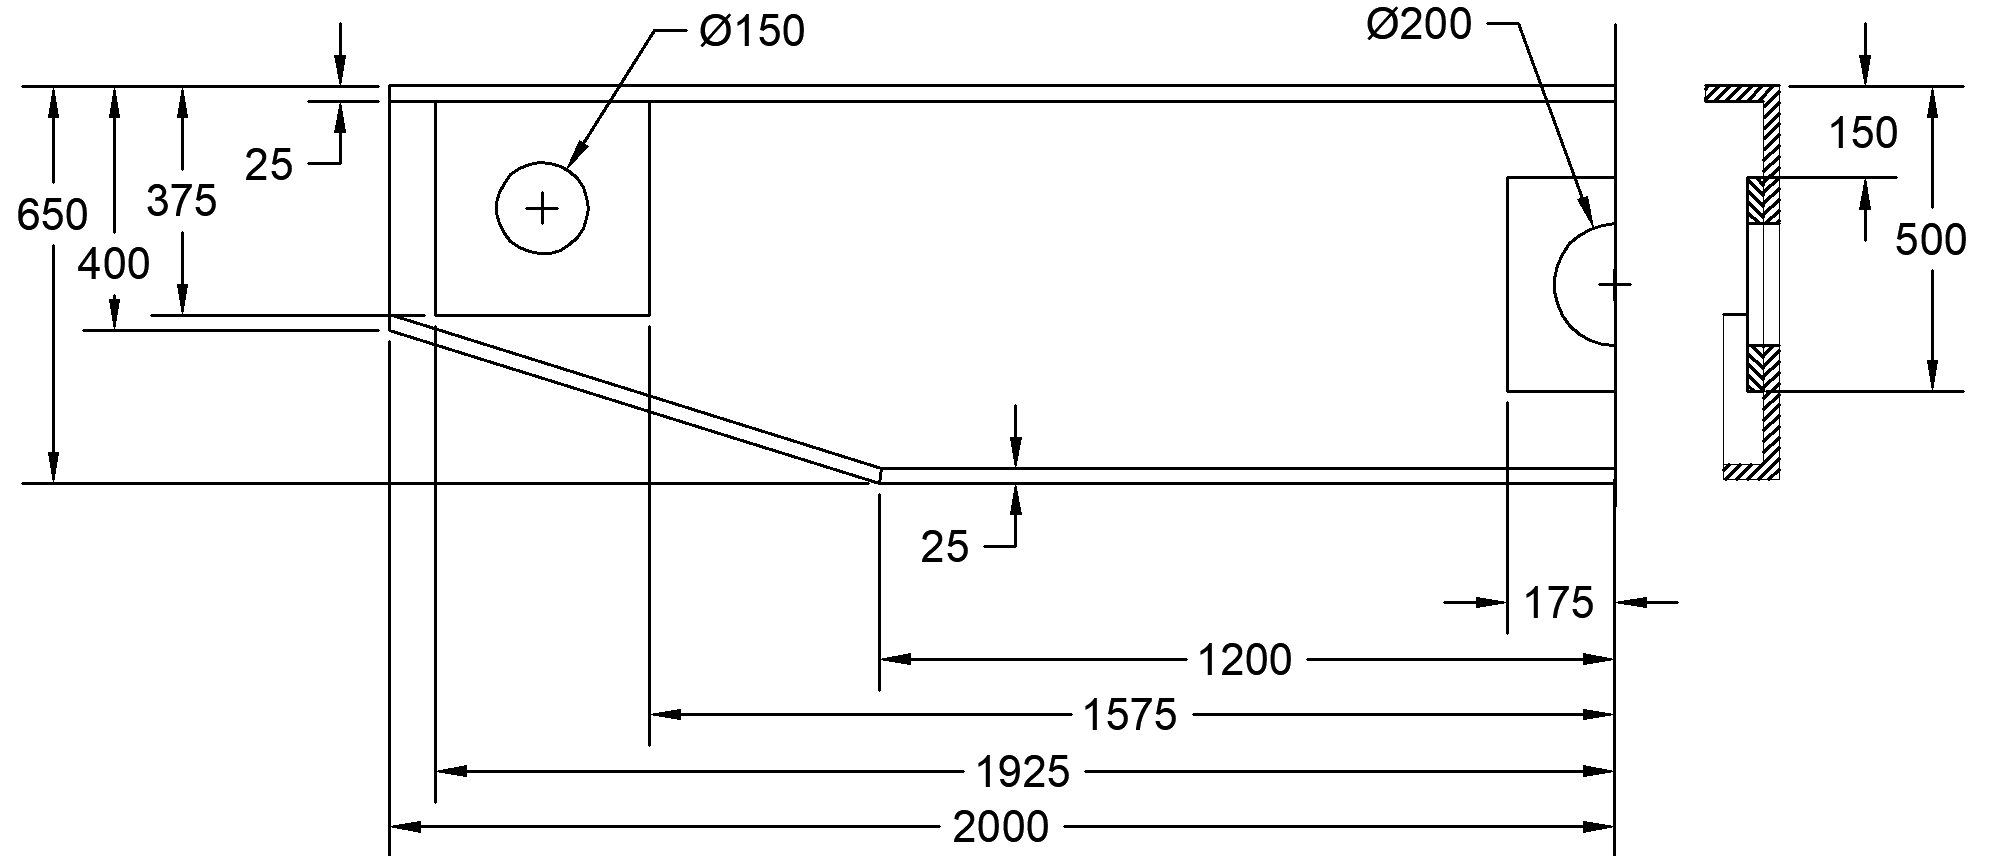
\includegraphics[width=\textwidth]{img/dim_beam.png}
	\label{img:dim_beam}
	\caption{Fixed Dimensions for the Example System Beam}
\end{figure}

Also fixed is the material, which is assumed to be ASTM A36 steel. The material has properties assumed to be: 

\begin{itemize}
\item Yield Strength: Mean 250MPa, Std. Deviation 32.5 MPa
\item Young's Modulus: 200 GPa
\end{itemize}

\subsection{Performance requirements}
In this case, performance requirements primarily relate to the lifting capacity and the allowable side pull on the beam. The requirements selected for this problem are: 
\begin{enumerate}
\item Lifting capacity: 60 metric tons, 60,000kg, 132,000 lbm, 588 kN. For this problem, 600 kN was used. 
\item Minimum capable side load: $\pm 5^{\circ} $
\end{enumerate}

As will be discussed in detail later, the beam to be analyzed is symmetric on 2 planes. This allows for the model to consist of only one quarter of the beam under study. Additionally, It will be later clarified that the selected solution methods utilize stochastic methods to model the loading. 

\chapter{Solution Principals}
The solution code in this study relies on several principals that are complex enough to require separate attention prior to introducing the solution method itself. This chapter provides a brief introduction of selected major concepts used in the solution. Each concept is related to the actual solution in general terms.  

\section{Numerical Optimization}
Optimization is defined as ``a mathematical technique for finding a maximum or minimum value of a function of several variables subject to a set of constraints."\cite{opt-def} In the specific case of engineering design, one of several techniques is used to find local or global extrema of a function of one or multiple variables. These techinques use various criteria to traverse the independent variables and detect these extrema. The method the optimizer uses to traverse the solution space has a significant impact on the speed at which the operation converges to a solution or solutions.\cite{basic-optim} \todo{Is this section complete enough?}

\todo{Introduce the concept of the objective function}
\subsection{Differential Evolution}
Differential evolution was selected as the optimizer for this study. 

Differential Evolution is a member of optimizers collectively known as \emph{Evolutionary Algrorithms}. These optimizers use various approaches to emulate the concept of biological evolution to optimize a given objective function. Differential optimization performs this task through the use of a 4-phased approach: Initialization, Mutation, Crossover, and Selection. \cite{diff-evol}

\subsubsection{Initialization}
Prior to starting the optimization loop, an initial ``population" of individuals has to be generated for the optimizer to work from. An individual consists of a vector $\vec{x}$ of values of the objective function's independent variables. The Initialization process generates a vector $\vec{X} = \left\{\vec{x}_1, \vec{x}_2 \cdots \vec{x}_n\right\}$ of individuals by randomly selecting values for the independent variables. This vector represents the complete population that will be operated on in the first generation of the optimization loop. These individuals will be collectively be known as \emph{parents}.\cite{diff-evol} 

In the case of the implementation presented here, Latin Hypercube Sampling (LHS) was employed to generate the random values to assemble $\vec{X}$. More detail on LHS can be found in section \ref{sec:lhs}. 

\subsubsection{Mutation}
The mutation operator is the first step for each cycle of the optimization loop. This algorithm emulates random mutations in genetic code commonly found in nature. Taking each individual from the vector of parents, a mutated vector of properties is generated. These vectors are known as \emph{trial vectors}. To perform this action, the basic process flow shown below is employed \cite{diff-evol}:

\
\begin{lstlisting}[caption=Pseudocode for the Mutation Operator \cite{diff-evol},captionpos=b]
trial_vector = empty_2d_vector[num_individuals][num_design_vars]
for integer j in [0 ... num_individuals]:
    x_1 = individuals[j]
    x_2 = random_member_of_individuals
    x_3 = random_member_of_individuals
    beta = x.x // (arbitrary amplification factor selected by user)
    for integer i in [0 ... num_design_vars]:
	    trial_vector[j][i] = x_1[i] + beta * (x_2[i] - x_3[i])
return trial_vector
\end{lstlisting}

This set of trial vectors is one of the distinguishing facets of Differential Evolution. If the equation on line 8 above is reviewed carefully, it can be seen that the trial vector is different than its associated parent vector by the distance between 2 other random individualswithin the solution space. This has the interesting effect of causing the differences to between parent and trial vectors to change based on the condition of the solution. Early in the solution process when the individuals are sparsely spaced across the solution space, the trial individuals tend to spread apart similarly. In later cycles as minima start to become identified, the distance between individuals becomes smaller. This has the effect of making the trial vectors land more closely to their associated parents. This allows Differential evolution to converge relatively quickly once minima start to appear in the solution space \cite{diff-evol}.

\subsubsection{Crossover}
The crossover operator combines the parent individuals and their associated trial individuals to make a single set of \emph{child individuals}. It does this using the following general procedure \cite{diff-evol}:

\begin{lstlisting}[caption=Pseudocode for the Crossover Operator \cite{diff-evol},captionpos=b]
child_vector = empty_2d_vector[num_individuals][num_design_vars]
for integer j in [0 ... num_individuals]:
    C = x.x //Constant that dictates how often the crossover picks from the trial vector. 
    for integer i in [0 ... num_design_vars]:
        rnd = make_random_number()
	if rnd > C
	    child_vector[j][i] = trial_vector[j][i]
	else
	    child_vector[j][i] = parent_vector[j][i]
return child_vector
\end{lstlisting}

\subsubsection{Selection}\todo{Flesh out these sections!}


\subsection{Extending DE to Multi-Objective}
Differential Evolution Optimization is originally a single-objective method. However, it can easily be extended to multi-objective operation by changing the method by which fitness is evaluated. Instead of a single fitness function, multiple independent fitness functions are evaluated using the concept of Pareto dominance. 

\todo{Complete this section}

\subsection{Pareto Dominance}
Pareto Dominance is a simple way to compare systems based on multiple different fitness criteria. Pareto dominance for a minimization problem can be described by the following formula: 

Let the vector of fitness values for two arbitrary solutions be defined as:
\begin{align*}
C_a &= 4
\end{align*}

$$
P_{a,b} = \begin{cases}
          \hbox{True  when  } C_{a}^i < C_{b}^i \; \forall i \in \{1..n\}\\ 
          \hbox{False otherwise}
          \end{cases}
$$

\todo{Section incomplete}

\section{Random Loads}
This study presents two different approaches for performing MODE optimization on finite element models. The key difference in how the two methods work is the choice of how the random loads in the problem are handled. In this section, the two strategies for generating random loads are introduced. 
\section{Latin Hypercube Sampling}
\label{sec:lhs}

Latin hypercube sampling is used throughout the code presented here to generate evenly distributed random data. this method of sampling was selected due to its ability to evenly spread out the sampling points throughout the variable's domain. It does this by programmatically ensuring that each value of each input variable is only represented once. It does this by separating the domain of each input variable into a predetermined number of strata, each with an identical probability of containing an arbitrary sample point. Then, one sample is taken from each of the strata. In this implementation, the different variables in the space do not interact, and the given random values of each input variable are combined at random to form a vector of input variables, also known as an individual \cite{lhs}.  

\subsection{The Reliability Index}
\label{sec:beta}
The reliability index is a unitless constant that can be used to infer the probability of a system or component to fail in service. Roughly, the Reliability index describes the safety factor of a system as the Z-score of a standard normal distribution, where higher numbers indicate higher probabilities of success. It is derived from the basic concept of probability of failure. 

Consider the following definition for the margin of safety for a system under stress \cite{struct-rel}:

\begin{equation}
Z = S_y - \sigma
\end{equation}
where:
\begin{align*}
S_y &= \text{Material Yielding Stress}\\
\sigma &= \text{Von Mises Stress resulting from the applied Load}
\end{align*}
If ``failure" is defined as \cite{struct-rel}:

\begin{align}
G\left( S_y, \sigma\right) &= S_y - \sigma \le 0\nonumber\\
G\left( S_y, \sigma\right) &= Z < 0
\end{align}
If we treat $Z$ as a random variable with a Gaussian distribution, The probability of failure occurring ($P_f$) is given as \cite{struct-rel}:

\begin{align}
P_f = P(Z<0) &= \Phi \left( \frac{0 - \mu_Z}{\sigma_Z}  \right)\nonumber\\
P_f &= 1 - \Phi \left( \frac{\mu_Z}{\sigma_Z} \right)\nonumber\\
P_f &= 1 - \Phi \left( \beta \right)\label{eq:Pf}
\end{align}
where:
\begin{align*}
\mu_Z &= \text{Mean of Z}\\
\sigma_Z &= \text{Standard Deviation of Z}\\
\Phi(x) &= \text{The CDF of the Normal (Gaussian) Distribution}
\end{align*}
From the above, it is clear we have defined $\beta$ as:

\begin{equation}
\beta = \frac{\mu_Z}{\sigma_z}\label{eq:protobeta}
\end{equation}
For the random variable $Z$, the mean and standard deviation are \cite{risk2}:
\begin{align}
\mu_Z &= \mu_{Sy} - \mu_\sigma\label{eq:muZ}\\
\sigma_Z &= \sqrt{\sigma_{\sigma}^2 + \sigma_{Sy}^2}\label{eq:sigmaZ}
\end{align}
where
   \begin{align*}
	   \mu_{Sy} &= \text{Mean of} S_y\\
	   \sigma_{Sy} &= \text{Std. Deviation of }S_y\\
	   \mu_{\sigma} &= \text{Mean of }\sigma\\
	   \sigma_{\sigma} &= \text{Std. Deviation of }\sigma
   \end{align*}
Substituting Equations \ref{eq:muZ} and \ref{eq:sigmaZ} into Equation \ref{eq:protobeta} yields:
   \begin{equation}
	   \beta = \frac{\mu_{Sy} - \mu_\sigma}{\sqrt{\sigma_{\sigma}^2 + \sigma_{Sy}^2}}
	   \label{eq:beta}
   \end{equation}

Equation \ref{eq:beta} represents the Reliability Index. This is the primary metric used to measure reliability in the Stochastic Loads method presented here. If we define reliability as \cite{risk2}: 

\begin{equation}
R = 1 - P_f
\end{equation}
The relation between $\beta$ and Reliability is clearly given from Equation \ref{eq:Pf}:
\begin{align}
R &= 1 - \left(1 - \Phi (\beta)\right)\nonumber\\
&= \Phi(\beta)
\end{align}
For example, for a value of $\beta$ of 1.96, the reliability is calculated as 97.5\%. For a $\beta$ value of 2.58, reliability rises to 99.5\%. 

In order to evaluate $\beta$ for the designs presented in this study, Equation \ref{eq:beta} will be used. To satisfy all the variables in this equation, the mean and standard deviation for both the material yield criterion and the applied Von Mises stress must be found. The properties related to properties of the material the object is made from are given assumed values that will be held constant across all designs. The stress-related properties, however, must be calculated.

\subsubsection{Finding $\mu_\sigma$ and $\sigma_\sigma$}
If $g(x_1, x_2, ... x_n) = Y$ denotes a function of multiple random variates and a single, dependent variable, let \cite{taylor}:
   \begin{align}
	   \mu(Y) = g(x_1, x_2, ... x_n) + \frac{1}{2} \sum_{i=1}^{n}\left( \frac{\partial^2 g}{\partial x_i^2} \sigma_{xi}^2  \right)
	            \label{eq:mu}\\
	   \sigma^2(Y) = \sum_{i=1}^{n}\left( \frac{\partial g}{\partial x_i} \sigma_{xi}  \right)^2 + 
			 \frac{1}{4} \sum_{i=1}^{n}\left( \frac{\partial^2 g}{\partial x_i^2} \sigma_{xi}^2  \right)^2 \label{eq:sigma}
   \end{align}
In our case, the term $Y$ will be the Von Mises Stress of our beam system. The tensor definition of the Von Mises stress at a given location can be written as:
   \begin{equation}
      \sigma = \sqrt{\frac{3}{2} \cdot \left(\sigma_{dev}:\sigma_{dev} \right)}
	\label{eq:basedef}
   \end{equation}
Where $\sigma_{dev}$ is the stress deviator tensor, which will be more completely addressed later. 
We can simplify derivation of equation \ref{eq:basedef} by hiding the tensor contraction in the equation with a placeholder variable:
   \begin{align}
	   \alpha = (\sigma_{dev}:\sigma_{dev})
	   \label{eq:defalpha}
   \end{align}
This turns equation \ref{eq:basedef} into:
   \begin{align}
      \sigma' = \sqrt{\frac{3}{2} \cdot \left(\alpha\right)}
   \end{align}
This simplified equation can be derived as shown below: 
   \begin{align}
	   \frac{\partial \sigma'}{\partial P_x} &= \sqrt{\frac{3}{2}} \left[\frac{1}{2} \frac{\partial \alpha}{\partial P_x} 
						    \left( \alpha \right)^{-\frac{1}{2}}\right]\label{eq:fd_vmx}\\
	   \frac{\partial^2 \sigma'}{\partial P_x^2} &= \sqrt{\frac{3}{2}} \left[ \frac{1}{2}  \frac{\partial ^2 \alpha}{\partial P_x^2}
	                                                \left( \alpha \right)^{-\frac{1}{2}} - 
							\frac{1}{4}  
							\left(\frac{\partial \alpha}{\partial P_x}\right)^2
							\left( \alpha \right)^{-\frac{3}{2}}\right] \\
	   \frac{\partial \sigma'}{\partial P_y} &= \sqrt{\frac{3}{2}} \left[\frac{1}{2} \frac{\partial \alpha}{\partial P_y} 
						    \left( \alpha \right)^{-\frac{1}{2}}\right]\\
	   \frac{\partial^2 \sigma'}{\partial P_y^2} &= \sqrt{\frac{3}{2}} \left[ \frac{1}{2}  \frac{\partial ^2 \alpha}{\partial P_y^2}
	                                                \left( \alpha \right)^{-\frac{1}{2}} - 
							\frac{1}{4}   
							\left(\frac{\partial \alpha}{\partial P_y}\right)^2
							\left( \alpha \right)^{-\frac{3}{2}}\right] \label{eq:sd_vmy}
   \end{align}
Of course, this introduces derivatives of $\alpha$ as values that must be calculated. In order to calculate these derivatives, the concept and application of the deviator tensor must be investigated further.


The Deviatoric Stress Tensor (or deviator tensor) describes the component of stress that tends to deform an element. It is given in terms of the overall stress tensor $\sigma'$ as: 
   \begin{equation}
      \sigma_{dev} = \sigma' - \frac{1}{3} \mathrm{tr}(\sigma') \left[ \mathbf{I} \right]
   \end{equation}
For purposes that will become clear later, we can call this operation a matrix operator $\gamma$:
   \begin{align}
      \gamma(x) &= x - \frac{1}{3} \mathrm{tr}(x) \left[ \mathbf{I} \right]\label{eq:gamma}\\
      \sigma_{dev} &= \gamma(\sigma') \nonumber
   \end{align}
In this study, $\sigma'$ is constructed from the component response tensors, $\sigma_{Px}$ and $\sigma_{Py}$. These are tensors that correspond to the stresses in the material when a unit load is applied in the x- and y- directions, respectively. These tensors can be used to define $\sigma'$:
   \begin{equation*}
      \sigma' = \sigma_{Px} \cdot P_x + \sigma_{Py} \cdot P_y
   \end{equation*}
Applying equation \ref{eq:gamma} to the above definition of $\sigma'$ yields:
   \begin{align}
	   \gamma_(\sigma') &= \left(\sigma_{Px} \cdot P_x + \sigma_{Py} \cdot P_y\right) - 
                       \frac{1}{3} \mathrm{tr} \left(\sigma_{Px} \cdot P_x + \sigma_{Py}
                       \cdot P_y\right) \left[ \mathbf{I} \right] 
   \end{align}
From here, it is important to remember that taking the trace of a matrix is a distributive operation, as is multiplying a scalar and a matrix. Therefore, the above equation can be rewritten as: 
   \begin{align}
	   \gamma(\sigma') &= \left(\sigma_{Px} \cdot P_x + \sigma_{Py} \cdot P_y\right) - 
                       \frac{1}{3} \left(\mathrm{tr} \left(\sigma_{Px} \cdot P_x\right) +
                       \mathrm{tr} \left( \sigma_{Py} \cdot P_y\right)\right) 
                       \left[ \mathbf{I} \right]\nonumber \\
                      &= \left(\sigma_{Px} \cdot P_x + \sigma_{Py} \cdot P_y\right) - 
		       \frac{1}{3} \left(\mathrm{tr} \left(\sigma_{Px} \cdot P_x\right)
		       \left[ \mathbf{I} \right] +
                       \mathrm{tr} \left( \sigma_{Py} \cdot P_y\right) 
                       \left[ \mathbf{I} \right]\right)\nonumber\\
		      &= \left(\sigma_{Px} \cdot P_x + \sigma_{Py} \cdot P_y\right) - 
		       \frac{1}{3} \left(P_x \cdot \mathrm{tr} \left(\sigma_{Px}\right)
		       \left[ \mathbf{I} \right] +
                       P_y \cdot \mathrm{tr} \left( \sigma_{Py} \right) 
                       \left[ \mathbf{I} \right]\right)\nonumber\\
		      &= P_x \cdot \left( \sigma_{Px} - \frac{1}{3} \mathrm{tr}(\sigma_{Px})
			 \left[ \mathbf{I} \right] \right) + P_y \cdot \left( \sigma_{Py} -
			 \frac{1}{3} \mathrm{tr}(\sigma_{Py})
			 \left[ \mathbf{I} \right] \right)\nonumber\\
		      &= P_x \cdot \gamma(\sigma_{Px}) + P_y \cdot \gamma(\sigma_{Py})
   \end{align}
Note that the terms $\gamma(\sigma_{Px})$ and $\gamma(\sigma_{Py})$ do not contain any terms related to $P_x$ or $P_y$. This implies that they are constant when deriving with respect to these variables. From this point forward, we will refer to these deviatoric unit tensors as:

   \begin{align*}
	   \gamma(\sigma_{Px}) &= \sigma_{devx}\\
	   \gamma(\sigma_{Py}) &= \sigma_{devy}
   \end{align*}
This means: 
   \begin{equation}
	   \sigma_{dev} = \sigma_{devx} \cdot P_x + \sigma_{devy} \cdot P_y
   \end{equation}

Returning to equation \ref{eq:defalpha}, we can begin to define $\alpha$ in terms of these new tensors. To start with, we need to breakdown the ``:" operator in the equation. This is the tensor contraction operator, and is defined as: 
   \begin{equation}
	   \left[A\right] : \left[B\right] = \mathrm{tr}(\left[A\right]\left[B\right])
	   \label{eq:tensorcont}
   \end{equation}
Because both matrix multiplication and the trace of a matrix are both distributive, the tensor contraction operator is also distributive. Using the definition in \ref{eq:tensorcont} and applying it to \ref{eq:defalpha} yields: 
   \begin{align}
	   \alpha &= \mathrm{tr}\left[(\sigma_{devx} \cdot P_x + \sigma_{devy} \cdot P_y) \cdot
		    (\sigma_{devx} \cdot P_x + \sigma_{devy} \cdot P_y)\right]\nonumber\\
		  &= \mathrm{tr}\left[\sigma_{devx} \cdot \sigma_{devx} \cdot P_x^2 + \left( 
		     \sigma_{devx} \cdot \sigma_{devy} + \sigma_{devy} \cdot \sigma_{devx} \right) \cdot P_x P_y + 
		     \sigma_{devy} \cdot \sigma_{devy} \cdot P_y^2 \right]\\
		  &= \mathrm{tr}\left[ \sigma_{devx} \cdot \sigma_{devx} \right] \cdot P_x^2 +  
		     \mathrm{tr}\left[ \sigma_{devx} \cdot \sigma_{devy} + \sigma_{devy} \cdot \sigma_{devx} \right]
                     \cdot P_x P_y + \mathrm{tr}\left[ \sigma_{devy} \cdot \sigma_{devy}\right] \cdot P_y^2
   \end{align}
Note that the center term is arranged as shown due to the non-commutative nature of matrix multiplication.
Now, we can take this definition of $\alpha$ and easily find the derivatives we need.
   \begin{align}
	   \frac{\partial \alpha}{\partial P_x} &= 
	   	\mathrm{tr}\left[\sigma_{devx} \cdot \sigma_{devx}\right] \cdot 2P_x + \mathrm{tr} \left[ 
		     \sigma_{devx} \cdot \sigma_{devy} + \sigma_{devy} \cdot \sigma_{devx} \right] \cdot P_y\label{eq:fd_ax}\\
	   \frac{\partial^2 \alpha}{\partial P_x^2} &=
	   	\mathrm{tr}\left[ \sigma_{devx} \cdot \sigma_{devx} \right] \cdot 2\\
	   \frac{\partial \alpha}{\partial P_y} &= 
	   	\mathrm{tr}\left[\sigma_{devy} \cdot \sigma_{devy}\right] \cdot 2P_y + \mathrm{tr} \left[ 
		     \sigma_{devx} \cdot \sigma_{devy} + \sigma_{devy} \cdot \sigma_{devx} \right] \cdot P_x\\
	   \frac{\partial^2 \alpha}{\partial P_x^2} &=
		\mathrm{tr}\left[\sigma_{devy} \cdot \sigma_{devy} \right]\cdot 2\label{eq:sd_ay}
   \end{align}

   With equations \ref{eq:fd_ax} through \ref{eq:sd_ay} coupled with equations \ref{eq:fd_vmx} through \ref{eq:sd_vmy}, we have all of the terms needed to construct and solve equations \ref{eq:mu} and \ref{eq:sigma}, substituting the equation for $\sigma$ into $Y$ for both equations. It is then easy to substitute the results of equations \ref{eq:mu} and \ref{eq:sigma} into \ref{eq:beta} and determine $\beta$.  In the code presented with this report, all of these terms are assembled separately and combined. Therefore, the final equation with all substitutions performed will not be shown here.

\subsubsection{Validating the derivation for $\mu_\sigma$ and $\sigma_\sigma$}
The equations for finding $\mu_\sigma$ and $\sigma_\sigma$ were validated by comparing the results from the equation to a Monte Carlo Simulation of the equation system. One of the test systems used was the following states of stress:

The mean and standard deviation of the input loads to the material was assumed to be:
\begin{align*}
    \mu_{px} &= 25 &\sigma_{px} &= 3.25\\
    \mu_{py} &= 150 &\sigma_{py} &= 19.5\\
\end{align*}

The unit response to stress was assumed to be: 
\begin{align*}
    U_{xpx} &= 2500  &U_{ypx} &= 750  &U_{xypx} &= 320\\
    U_{xpy} &= 250  &U_{ypy} &= 7500  &U_{xypy} &= 210
\end{align*}

The above unit responses can be represented as tensors. These tensors are: 

\begin{align*}
\mathbf{U}_{px} &= \left[ 
\begin{matrix}
2500 & 320 & 0\\
320 & 750 & 0\\
0 & 0 & 0
\end{matrix}
\right]
&\mathbf{U}_{py} &= \left[
\begin{matrix}
250&210&0\\
210&7500&0\\
0&0&0
\end{matrix}
\right]
\end{align*}

The deviators of these tensors are: 

\begin{align*}
\mathbf{\sigma}_{devx} &= \left[ 
\begin{matrix}
1416.67 & 320 & 0\\
320 & -333.3 & 0\\
0 & 0 & -1083.33
\end{matrix}
\right]
&\mathbf{\sigma}_{devy} &= \left[
\begin{matrix}
-2333.3&210&0\\
210&4916.67&0\\
0&0&-2583.33
\end{matrix}
\right]
\end{align*}

A Monte Carlo simulation was prepared using the properties above. A sample size of $1.5\times 10^6$ was used for the simulation. Then, code was created based on the equations \ref{eq:mu} and \ref{eq:sigma}, as well as \ref{eq:fd_ax} to \ref{eq:sd_ay}. This code was run with the same parameters, and results obtained. The results from these two analyses can be seen in Table \ref{tab:val_tensors} below. 

\begin{table}[!hbtp]
\caption{Selected Validation Results for the Taylor Approximation for finding $\mu_\sigma$ and $\sigma_\sigma$}
\small
\label{tab:val_tensors}
\begin{center}
\begin{tabular}{|l|p{2.1cm}|p{2.5cm}|p{2.5cm}|}
\hline
& Monte Carlo Simulation & Taylor Expansion Approximation & Error percentage\\
\hline
Expected Value (Mean) & $1.0993 \times 10^6$ & $1.0994 \times 10^6$ & $-3.9552 \times 10^{-4} \;\%$\\
Standard Deviation & $1.4382 \times 10^5$ & $1.4386 \times 10^5$ & $-3.2071 \times 10^{-2} \;\%$\\
\hline
\end{tabular}
\end{center}
\end{table}

Based on this table, it is plainly apparent that the tensor-based Taylor Series Approximation for finding $\mu_\sigma$ and $\sigma_\sigma$ is an appropriate approximation method. The code that was developed for the validation is identical to the code in the final product in the main analysis loop. 


\section{Finite Element Modeling}

When performing optimization to find designs, numerous designs must be analyzed and evaluated for fitness. In some cases, these designs and their fitness functions can be modeled using closed form equations. In the many cases, however, the designs are complex enough that finding closed form models of their behavior is infeasible. In the case that no closed form solutions can be found, numerical analysis can offer an alternative method of evaluating for fitness. 

For this study, numerical analysis in the form of Finite Element Modeling was chosen as the method for evaluating the designs for fitness. Each design and load case each are represented as slight modifications to a basic model file containing the fixed geometry and ``starting" parameters for the design and loading variables.  \todo{Do I need to summarize the basics of finite element modeling?}

This study makes exclusive use of quadrilateral shell elements, known to NASTRAN as \codeword{CQUAD4} elements. These elements are 2-dimensional, but do model deformation in all thee dimensions. However, an important assumption made by using these elements is that the entire thickness of the plate distributes the stress applied to the element equally. This implies that deformations in the thickness direction cannot be modeled this way. For example, if a plate can buckle or bend through its thickness this type of element would not be suitable. This model makes use of these elements for the beam flanges, but the elements are oriented to be coplanar with the beam web. This means the flange width is modeled as plate thickness. This orientation will not detect local flange effects such as buckling or local bending. However, this study is primarily concerned with failure of the gross section. Due to the system geometry, these stresses are negligible and therefore the model's inability to properly model them does not appreciably affect the accuracy of this model. This modeling strategy also has the advantage of simplifying the alteration of the flange thickness programmatically. 

\subsection{Selected Model}

\begin{figure}
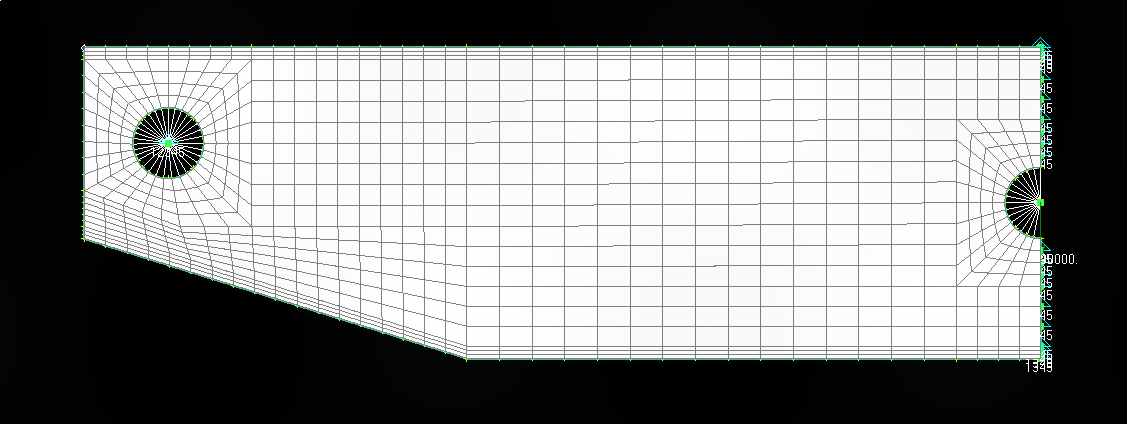
\includegraphics[width=\textwidth]{img/mesh_geom.png}
\caption{Mesh Geometry as shown in Siemens Femap}
\label{img:mesh_geom}
\end{figure}

The model developed for the example problem considered in this work is shown in figure \ref{img:mesh_geom}. This model was developed using the dimensional data shown in figure \ref{img:dim_beam}. As shown, the model consists of several regions, all of which are modeled using \codeword{CQUAD4} elements. The regions that are of importance for this study are: 

\begin{enumerate}
  \item The top flange
  \item The bottom flange
  \item The web
  \item A thickened region surrounding the hoist mounting lug
  \item A thickened region surrounding the load mounting lug. 
\end{enumerate}

\begin{figure}
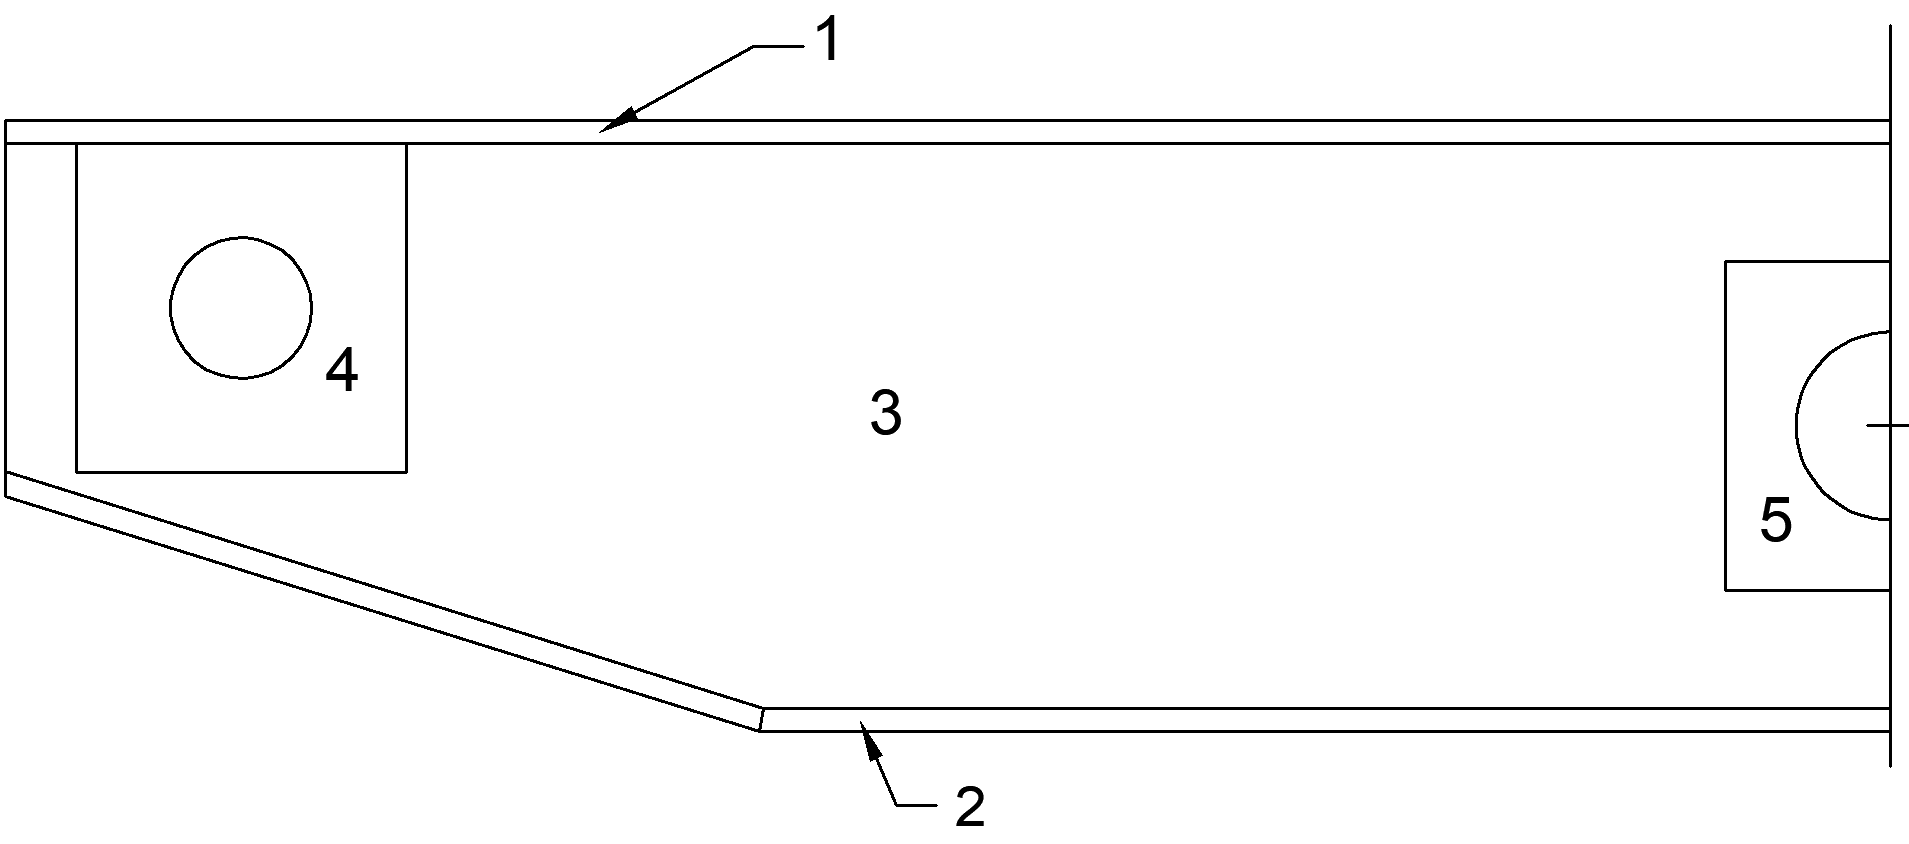
\includegraphics[width=\textwidth]{img/numbered_geom.png}
\caption{Diagram of modeled beam showing region numbers}
\label{img:num_geom}
\end{figure}

Figure \ref{img:num_geom} shows the named regions as they correspond to portions of the model/drawing. 

Also worth noting is that this model is a partial representation of the whole beam. As the example beam in figure \ref{img:basic_beam} shows, the beam features symmetry along the front view. Due to the typical construction of these beams, they also exhibit symmetry along the top view as well. Because of this, the model presented is only one quarter of the complete beam. To account for this, constraints are imposed along the symmetry cut that simulate the remainder of the beam. These constraints can be seen in figure \ref{img:mesh_geom} as symbols along the right edge of the diagram. These constraints are along model axes 1, 3, 4, and 5. This equates to constraining X and Z translation, as well as X and Y rotations. This simulates a moment bearing connection at the center of the beam. This is a commonly accepted way of simulating symmetry in NASTRAN\todo{Needs Citation}. 


\chapter{Tools and Software Used}
%Tools and Software Used. 
For this study several externally developed or commercially purchased tools, hardware, and software were used. Each major tool or piece of hardware will be briefly introduced and given a brief description of its source, purpose and method of procurement.

\section{Computing Hardware}
\todo{Cite the spec sheet for These parts!}The analyses presented in this report were obtained using commercially available computing hardware. The computer's relevant specifications are given below: 

\begin{itemize}
\item CPU: AMD Ryzen 2400G. 4 Processing Cores with 8 execution threads. Frequency during tests: 3.8GHz
\item Memory: 16GB DDR4 Memory at a frequency of 2666 MHz
\item Storage: Intel 540 Series SSD. Capacity:240GB, up to 540 MBps read speed, 490 MBps write
\end{itemize}

While this computer is a general purpose unit and sees daily use outside the scope of this report, no other tasks were performed simultaneously with the workloads presented herein. Execution times presented represent near-maximum performance for these workloads. 

\section{Software}

\chapter{Solution Methods}
With all of the principals having been covered previously, the actual solution methodology can be discussed. This chapter provides an overview of the actual solution process used in the code that was developed. While it does not provide a full analysis and discussion of the entire codebase, it should provide sufficient information for the reader to understand the actual code provided. 

\section{Modeling the base beam}
For both solution methods, a common basic design of the beam to be studied was constructed. For this study, a basic design using two ``C"-style sections to form the two main moment-bearing sections was selected. This style was selected because the cross section lends itself to parameter-based optimization, whereas more complex designs such as box beam spreaders are more well suited to full geometry optimization. Section \ref{sec:beam_des} has details on the design. 

This basic design was modeled in Siemens's Finite Element Pre-processor, FEMAP. The modeled area takes advantage of the two-plane symmetry in the beam to only model one quarter of the beam. It is worth noting that the loading on the beam is affected by the symmetry, and the loads presented for analysis are one fourth of the actual beam loadings. 

\section{Solution Strategies}
Two solution strategies were attempted for the example problem proposed. One was termed as the \emph{Aggregated Latin Hypercube Sampling Approach}, while the other was named the \emph{Stochastic Loads Approach}. The following sections describe each solution method in detail and outline similarities and differences between them. 

\subsection{Aggregated Latin Hypercube Approach}

In a nutshell, the Aggregated Latin Hypercube (ALHS) Approach analyzes a variety of discrete load cases and collects Pareto Front data for each load case. It does this by:

\begin{enumerate}
\item Identifying Load Cases to consider
\item Performing MODE Optimization for each identified load cases. This generates a unique Pareto Front for each load case. 
\item Aggregating the Pareto Fronts from all load cases to find the overall best designs across all load cases. 
\end{enumerate}
Each individual step of this process is outlined in detail below. 

\subsubsection{Identify Load Cases}
In order to find load cases for use, a Latin Hypercube Sampling algorithm is used to select 1000 independent loading conditions within the set of possible load conditions, which is assumed to be a set of normally distributed sample spaces. In this case, the most conservative loadings are those significantly above the mean for the magnitude of the applied force. In order to ensure reliability, the set of load cases to be analyzed is restricted to those load cases more than 1.96 standard deviations above the mean value of the applied load. This ensures that all of the load cases considered are in the top 2.5\% of the sample space. This will result in a set of approximately 25 load cases to consider. 
\subsubsection{Analyze load Cases} 
For each load case selected, a set of 50 randomly selected candidate designs are generated. These designs are analyzed using Finite Element Analysis to find the maximum stress and design weight. These values are used as fitness functions to rank the designs. This process is repeated using a Multi Objective Differential Evolution algorithm to selectively refine the designs for a set number of generations.
\subsubsection{Aggregation}
At this point, the solution algorithm has 25 separate load cases with individual Pareto fronts. The designs that make up each Pareto front are added to a single unified set of designs. From there, they are once again ranked according to dominance in accordance with Equation \ref{eq:dominance} and a ``final" Pareto front is generated. The designs that comprise this ``final" Pareto front are considered to be the most desirable designs and are presented to the designer.

\subsection{Stochastic Loads Approach}
The stochastic loads approach is functionally similar to the Aggregated Latin Hypercube Sampling Approach, with a few key differences: 

\begin{enumerate}
\item Only a single load case is considered. 
\item Stress is not directly considered a fitness variable. Instead, the Reliability Index is considered. While the Reliability Index is proportional to stress, it is not a direct measurement. See Section \ref{sec:beta} for details. 
\end{enumerate}
The overall process is detailed below. 

\subsubsection{Load Case}
Instead of using multiple load cases, this approach uses a single load case. However, it is specified as a stochastic set of loads instead of discrete loads applied. For example, the load case considered for the Example System is shown in Table \ref{tab:stoch_params}. Note that this information matches the design parameters given in section \ref{sec:perf_req}. Specifying the load case this way effectively covers the entire performance envelope and makes the single load case valid for all states of load on the beam. 

\begin{table}[!h]
    \begin{center}
    \begin{tabular}{|l|cc|}
	    \hline
	    Parameter & Mean Value & Standard Deviation\\
	    \hline
	    Hoist Load X Direction & 0N & 13kN\\
	    Hoist Load Y Direction & 150kN & 19.5kN\\
	    \hline
    \end{tabular}
    \caption{Stochastic Parameters for Example System}
    \label{tab:stoch_params}
    \end{center}
\end{table}

\subsubsection{Analyze Load Case}
The actual analysis of the load case selected is nearly identical to the ALHS Approach. The key difference is the use of the unitless parameter $\beta$ to represent the stress on the beam. This allows the stress, and by inference the safety factor of the device, to be represented in stochastic terms. As mentioned in section \ref{sec:beta}, the calculation for $\beta$ requires the two unit response tensors $\sigma_{Px}$ and $\sigma_{Py}$ to be retrieved. Currently, this must be done by running NASTRAN twice: Once with a unit load in the x direction, and again with a unit load in the y direction. For a complete discussion and derivation of the parameter $\beta$, see section \ref{sec:beta}. Using $\beta$ and the component weight as fitness measurements, MODE is performed on the load case.

\subsubsection{Reporting}
MODE optimization on the load case defined above generates a single Pareto Front that is reported to the user as recommended designs. Also reported is the Pareto Front presented graphically. 

\chapter{Selected Results}
\chapter{Concluding Remarks}
\printbibliography[title={References},heading=bibnumbered]
\chapter{Appendix A: Complete Code Listing}
\end{document}
